\documentclass[a4paper,12pt]{article}

\usepackage[czech]{babel}
\usepackage[utf8]{inputenc}
\usepackage{cmap}
\usepackage{graphicx}
\usepackage{amsopn}

\DeclareMathOperator{\Exp}{Exp}
\DeclareMathOperator*{\E}{E}

\title{Modelování směny pekárny s teorií hromadné obsluhy}
\date{semestrální práce}
\author{Tomáš Zikmund}

\begin{document}
\maketitle
\begin{abstract}
Zadání: Cílem práce je modelovat průběh směny v maloobchodě - v pekárně. 
\end{abstract}

\section{Exponenciální rozdělení}
\subsection{Poissonovo rozdělení}
Poissonovo rozdělení s parametrem \(\lambda > 0\) je dáno jako 
\[P(X = x) = \frac{\lambda^k}{k!}\exp(-\lambda).\]
Lze interpretovat tak, že náhodná veličina \(X\) Poissonova rozdělení představuje 
počet výskytu nějaké události v jistém časovém intervalu a parametr \(\lambda = \E X\). 

\subsection{Exponenciální rozdělení}
Exponenciální rozdělení s parametrem \(\lambda\) lze interpretovat jako dobu mezi výskyty dvou událostí, 
jejichž počet v pevném časovém intervalu odpovídá Poissonovu rozdělení s parametrem \(\lambda\). 
Hustota pravděpodobnosti je tvaru:
\[f(x) = \lambda \exp(-\lambda x),\qquad\mbox{pro~}x\geq 0.\]

Pro \(X\sim \Exp(\lambda)\) platí \(\E X = \frac{1}{\lambda}\).

\section{Modelování fronty v THO}
\subsection{Model s diskrétním časem}
Sledovaný časový úsek \(T\) se rozdělí na \(M\) malých intervalů \(\Delta t\). 
Následně se procházejí všechny malé intervaly \(\Delta t\) a zkoumá se, jestli v nich došlo k události
(příchod zákazníka, odchod obslouženého, \ldots). Důležité je volit časový krok tak, aby v každém kroku přišel 
nejvýše jeden zákazník. Frontu lze reprezentovat markovským procesem jako na obrázku \ref{fig:markowski}. 
%Podmínka existence stacionárního stavu je \(\lambda < n\mu\), kde \(\lambda\) je intenzita příchozích zákazníků, 
%\(\mu\) je intenzita obsluhy a \(n\) je počet přepážek. 

\begin{figure}[h]
\setlength{\unitlength}{0.99\columnwidth}
\begin{picture}(1,0.322)
\put(0,0.1){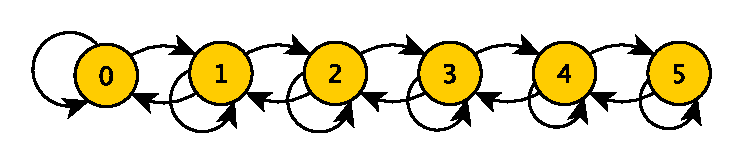
\includegraphics[width=\unitlength]{markowski.pdf}}
\small
\put(0,0.12){\rotatebox{90}{$1-\lambda\cdot\Delta t$}}
\put(0.17,0.28){$\lambda\cdot\Delta t$}
\put(0.10,0.10){\rotatebox{45}{$\mu\cdot\Delta t$}}
\put(0.33,0.28){$\lambda\cdot\Delta t$}
\put(0.29,0.09){\rotatebox{45}{$2\mu\cdot\Delta t$}}
\put(0.49,0.28){$\lambda\cdot\Delta t$}
\put(0.45,0.08){\rotatebox{45}{$3\mu\cdot\Delta t$}}
\put(0.65,0.28){$\lambda\cdot\Delta t$}
\put(0.60,0.08){\rotatebox{45}{$3\mu\cdot\Delta t$}}
\put(0.81,0.28){$\lambda\cdot\Delta t$}
\put(0.75,0.08){\rotatebox{45}{$3\mu\cdot\Delta t$}}
%\tiny
%\footnotesize
\scriptsize
\put(0.11,0.030){\rotatebox{45}{$1-(\mu+\lambda)\Delta t$}}
\put(0.27,0.016){\rotatebox{45}{$1-(2\mu+\lambda)\Delta t$}}
\put(0.44,0.014){\rotatebox{45}{$1-(3\mu+\lambda)\Delta t$}}
\put(0.59,0.020){\rotatebox{45}{$1-(3\mu+\lambda)\Delta t$}}
\put(0.74,0.020){\rotatebox{45}{$1-(3\mu+\lambda)\Delta t$}}
\Huge
\put(0.97,0.225){\ldots}
\normalsize
\end{picture}
\caption{Fronta THO jako markovský proces. Zákazníci přicházejí s paramtrem \(\lambda\) 
a můžou být obslouženi u jedné ze 3 přepážek. Doba obsluhy je popsána parametrem \(\mu\). 
Délka fronty jsou jednotlivé stavy markovského procesu. }
\label{fig:markowski}
\end{figure}

Nevýhodou tohoto přístupu je veliká nadbytečnost. Program prochází veliké množství kroků, 
ve kterých nedojde ke změně. Navíc neznáme přesnou dobu příchodu zákazníka a náročněji modelují 
další parametry, jako třeba \uv{trpělivost zákazníků}. 

\subsection{Model diskrétních událostí}
Tento model má náročnějsí algoritmus, na který můžeme nahlížet jako \uv{event-driven}. 
%\scriptsize
\footnotesize
\begin{verbatim}
# inicializace
t = 0 # vynuluj cas
prichod = exprand(1/zakazniciZaHodinu) # vygeneruj cas prichodu dalsiho zakaznika

# simulace
while t < dobaSimulace: # opakuj dokud cas nedosáhne celkove doby simulace
   # cas prichodu zakaznika je drive, nez konec obsluhy nebo netrpelivost
   if prichod < min(obsluha,odchod): 
      t = prichod # posun hodiny
      # novy zakaznik: jde rovnou k prepazce, nebo pocka ve fronte
      zakaznik = new Zakaznik()
      if size(vObsluze) < pocetPrepazek: # je volna prepazka
         zakaznik.konecObsluhy = t + exprand(dobaObsluhy) # urci se cas, kdy odejde
         vObsluze.pridej(zakaznik)
      else size(fronta) < maxDelkaFronty: # zakaznik musi do fronty 
         # urci se cas, do kdy zakaznik vydrzi ve fronte
         zakaznik.netrpelivyOdchod = t + exprand(dobaTrpelivosti) 
         fronta.pridej(zakaznik)

      # priprav cas prichodu dalsiho zakaznika
      prichod = t + exprand(1/zakazniciZaHodinu)

   elseif obsluha < odchod: # konec obsluhy nastane drive, nez netrpelivy odchod
      t = obsluha # posun hodiny

      odejdiHotovehoZakaznika()
      # vyberDalsihoZfronty
      zakaznik = fronta.prvni()
      zakaznik.konecObsluhy = t + exprand(dobaObsluhy) # urci se cas, kdy odejde
      vObsluze.pridej(zakaznik)

      # priprav cas dalsiho konce obsluhy
      obsluha = min(vObsluze) 

   else: # nastal okamzik kdy nektery zakaznik z fronty netrpelive odesel
      t = odchod # posun hodiny
      odejdiNetrpelivehoZakaznika()
      odchod = min(fronta) # pripravi se cas dalsiho odchodu
# konec simulace
\end{verbatim}
\normalsize

Takto napsaný model umožňuje sledovat, jakou dobu stráví zákazníci v obsluze a ve frontě. 
Dále můžeme zákazníkům přiřadit trpělivost při čekání ve frontě nebo obnos peněz, který hodlají 
utratit. 

\section{Popis modelu pekárny}
Do pekárny náhodně přicházejí zákazníci (počet zákazníků za hodinu). Zákazníci budou obslouženi 
u jedné z několika přepážek (doba obsluhy). Zákazníci chtějí utratit určité množtví peněz. Nejsou-li 
ihned obslouženi, čekají ve frontě, ale nejdéle jen po určitou dobu (doba trpělivosti). 

Budu sledovat v závislosti na počtu pokladních (přepážek) zisk během směny, zisk na jednu pokladní, 
dobu strávenou čekáním a počty neobsloužených zákazníků. 

\section{Formulace v termínech THO}
\subsection{Vstupní proud}
\begin{itemize}
	\item zdroj požadavků - nekonečný
	\item vstupní proud - náhodný (Poissonův tok), 100 zákazníků/hodina
\end{itemize}

\subsection{Fronta}
\begin{itemize}
	\item délka fronty - nekonečná
	\item timeout (trpělivost zákazníků ve frontě) - 15 minut
	\item disciplína čekání - FIFO
\end{itemize}
\subsection{Uzel obsluhy}
\begin{itemize}
	\item počet kanálů - 1 až 10
	\item doba obsluhy - náhodná (Poissonův tok), 2 minuty
\end{itemize}

\section{Existence ustáleného stavu}
Něchť \(p_k(t)\) značí pravděpodobnost, že v systému v čase \(t\) se nachází \(k\) požadavků (\(k\) lidí v pekárně). 
Pokud 
\[\forall k \qquad p_k = \lim_{t\to\infty} p_k(t),\]
hovoříme o ustáleném stavu. Lze ukázat, že pro systém s Poissonovým vstupním a výstupním tokem je nutnou 
podmínkou existence stacionárního stavu 
\[\lambda < n\mu,\]
kde \(\lambda\) je intenzita příchozích zákazníků, \(\mu\) je intenzita obsluhy a \(n\) je počet přepážek. 
Jinými slovy už intuitivně musí být výstup větší, než vstup.

Dále můžeme mít frontu s odmítáním. Příchozí zákazník je odmítnut, čeká-li ve frontě příliš lidí. 
Pravděpodobnosti konvergují, ale je nenulová pravděpodobnost, že zákazník nebude obsloužen. 
U Poissonových toků se asymproticky blíží hodnotě \(\max(0,1-\frac{n\mu}{\lambda})\). 

V modelu pekárny uvažujeme případ, že zákazníci ve frontě vydrží pouze nějakou dobu. V důsledku toho 
střední hodnota délky fronty nepřesáhne hodnotu 
\[\lambda \frac{\tau}{\Delta t}, \]
kde \(\tau\) je střední doba trpělivosti zákazníků, \(\Delta t\) je časová jednotka vstupní intenzity \(\lambda\). 

V obrázcích \ref{fig:fronta}, \ref{fig:frontaMax} a \ref{fig:frontaTO} je zobrazen vývoj počtu zákazníků ve frontě
v průběhu 16 hodin, pokud je vstupní tok \(\lambda = 100~\) zákazníků za hodinu a celkový výstupní tok je v rozsahu 50 až 150 
odbavených zákazníků za hodinu. 

\begin{figure}
\centering
\includegraphics[width=0.8\columnwidth]{fronta.pdf}
\label{fig:fronta}
\caption{Vývoj počtu zákazník ve frontě v průběhu 16 hodin. Fronta je bez omezení, vstupní tok \(\lambda = 100 \mbox{~h}^{-1}\). }
\end{figure}
\begin{figure}
\centering
\includegraphics[width=0.8\columnwidth]{frontaMax.pdf}
\label{fig:frontaMax}
\caption{Vývoj počtu zákazník ve frontě v průběhu 16 hodin. Fronta je omezena na maximálně \(20\) lidí, 
další jsou rovnou odmítnuti. Vstupní tok je \(\lambda = 100 \mbox{~h}^{-1}\). }
\end{figure}
\begin{figure}
\centering
\includegraphics[width=0.8\columnwidth]{frontaTimeout.pdf}
\label{fig:frontaTO}
\caption{Vývoj počtu zákazník ve frontě v průběhu 16 hodin. Fronta je bez omezení, ale zákazníci ve frontě 
vydrží v průměru 15 minut, pak odejdou neobslouženi. Vstupní tok je \(\lambda = 100 \mbox{~h}^{-1}\). }
\end{figure}

\section{Výsledky}
\subsection{Jedno pozorování}
Na obrázcích \ref{fig:jedenPrubeh} a \ref{fig:jedenPrubeh4} je zobrazen průběh jedné osmihodinové směny v pekárně. 
Vstupní tok je \(\lambda = 100\) zákazníků za hodinu a výstupní tok každé pokladny je \(\mu = 30\) zákazníků za hodinu, 
tedy průměrná doba obsluhy je 2 minuty. V prvním případě je pouze jedna pokladna a v druhém jsou pokladny čtyři. 
Zákazníci mají trpělivost vydržet ve frontě okolo 15 minut. 
Do modelu jsem přidal zákazníkům ochotu utratit okolo 100 Kč s gamma rozdělením. U zákazníků, kteří nebyli obslouženi počítám 
ušlý zisk. Po skončení směny jsou zákazníci čekající ve frontě z pekárny vykázáni bez obsloužení. 

\begin{figure}
\centering
\includegraphics[width=0.99\columnwidth]{jedenPrubeh.pdf}
\label{fig:jedenPrubeh}
\caption{Simulace jedné osmihodinové směny v pekárně s jednou pokladnou. Fronta je bez omezení, ale zákazníci ve frontě 
vydrží v průměru 15 minut, pak odejdou neobslouženi. Vstupní tok je \(\lambda = 100 \mbox{~h}^{-1}\). 
Průměrná doba strávená obsluhou u přepážky jsou 2 minuty s exponenciálním rozdělením. Výstupní tok 
jedné pokladny je tak \(\mu = 30 \mbox{~h}^{-1}\). Zákazníci mají ochotu v pekárně utratit v průměru 100 Kč s gamma rozdělením. 
Neobsloužení zákazíci tvoří ušlý zisk. Po skončení směny jsou zákazníci čekající ve frontě z pekárny vykázáni bez obsloužení.}
\end{figure}
\begin{figure}
\centering
\includegraphics[width=0.99\columnwidth]{jedenPrubeh4.pdf}
\label{fig:jedenPrubeh4}
\caption{Simulace jedné osmihodinové směny v pekárně se 4 pokladnami. Fronta je bez omezení, ale zákazníci ve frontě 
vydrží v průměru 15 minut, pak odejdou neobslouženi. Vstupní tok je \(\lambda = 100 \mbox{~h}^{-1}\). 
Průměrná doba strávená obsluhou u přepážky jsou 2 minuty s exponenciálním rozdělením. Výstupní tok 
jedné pokladny je tak \(\mu = 30 \mbox{~h}^{-1}\). Zákazníci mají ochotu v pekárně utratit v průměru 100 Kč s gamma rozdělením. 
Neobsloužení zákazíci tvoří ušlý zisk. Po skončení směny jsou zákazníci čekající ve frontě z pekárny vykázáni bez obsloužení.}
\end{figure}

\subsection{Více pozorování}
V tomto odstavci jsou prezentovány výsledky 100 pozorování. Je-li v systému ustálený stav, pak ten rozhoduje o výsledku simulace. 
Více pozorování tak pouze eliminuje přechodný děj prázdné pekárny do ustáleného stavu. 

Po otevření pekárny začnou chodit zákazníci. Existuje-li ustlený stav, pekárna do něj dokonverguje a střední hodnota délky fronty 
zůstává skoro jistě konstantní. Bez ustáleného stavu se fronta naplní čekajícími zákazníky, kteří jsou po zavření pekárny vykázáni 
bez obsloužení. Proto lze předpokládat, že bez ustáleného stavu budou střední hodnoty délky fronty mít veliký rozptyl daný především
vyprázdněním pekárny každých 8 hodin. 

\subsubsection{Fronta velmi trpělivých zákazníků bez omezení}
V tomto případě jsou jedinými parametry vstupní tok \(\lambda = 200\) zákazníků za hodinu a 
střední doba obsluhy 2 minuty (\(\mu = 30\) zákazníků za hodinu). Zákazníci z fronty neodcházejí 
pouze jsou odmítnutí po skončení směny. 

\begin{tabular}{c|r@{$\pm$}l|r@{$\pm$}l|r@{$\pm$}l|r@{$\pm$}l}
	\# pokladen & \multicolumn{2}{|c|}{Tržba} & \multicolumn{2}{|c|}{Doba čekání} & \multicolumn{2}{|c|}{Odmítnutí zák.} & \multicolumn{2}{|c}{Délka fronty}\\ \hline\hline	
	1 &   24000 & 2000  &  168     &  7      &  560   & 30    &  280    & 20    \\
	2 &   48000 & 2000  &   97     &  9      &  320   & 33    &  160    & 20    \\
	3 &   71000 & 2000  &   30     & 10      &   80   & 36    &   40    & 20    \\
	4 &   79000 & 3000  &    1.9   &  0.9    &    4   &  6    &    3    &  2    \\
	5 &   80000 & 3000  &    0.4   &  0.1    &    0   &  2    &    0.6  &  0.2  \\
	6 &   80000 & 3000  &    0.11  &  0.05   &    0   &  1    &    0.18 &  0.08 \\
	7 &   80000 & 3000  &    0.03  &  0.02   &    0.1 &  0.5  &    0.05 &  0.03 \\
	8 &   80000 & 3000  &    0.008 &  0.007  &    0.0 &  0.3  &    0.01 &  0.01 
\end{tabular}
\begin{figure}[h]
\centering
\includegraphics[width=0.99\columnwidth]{bezOmezeni.pdf}
\label{fig:bezOmezeni}
\caption{Simulace \(N=100\) směn v pekárně. Fronta je bez omezení.
Vstupní tok je \(\lambda = 100 \mbox{~h}^{-1}\). 
Průměrná doba strávená obsluhou u přepážky jsou 2 minuty s exponenciálním rozdělením. Výstupní tok 
jedné pokladny je tak \(\mu = 30 \mbox{~h}^{-1}\). Zákazníci mají ochotu v pekárně utratit v průměru 100 Kč s gamma rozdělením. 
Neobsloužení zákazíci tvoří ušlý zisk. Po skončení směny jsou zákazníci čekající ve frontě z pekárny vykázáni bez obsloužení.}
\end{figure}

\subsubsection{Fronta velmi trpělivých zákazníků maximální délky 20}
Zákazník je rovnou odmítnut, čeká-li ve frontě 20 lidí. Vstupní tok je \(\lambda = 200\) zákazníků za hodinu a
střední doba obsluhy 2 minuty (\(\mu = 30\) zákazníků za hodinu). Na konci směny jsou odmítnuti všichni. 

\begin{tabular}{c|r@{$\pm$}l|r@{$\pm$}l|r@{$\pm$}l|r@{$\pm$}l}
	\# pokladen & \multicolumn{2}{|c|}{Tržba} & \multicolumn{2}{|c|}{Doba čekání} & \multicolumn{2}{|c|}{Odmítnutí zák.} & \multicolumn{2}{|c}{Délka fronty}\\ \hline\hline	
	1 &   24000 & 2000  &   11.4   &  0.4    &  560   & 30    &  19.2  & 0.1  \\
	2 &   48000 & 2000  &   10.6   &  0.3    &  320   & 40    &  17.8  & 0.4  \\
	3 &   71000 & 2000  &    8     &  1      &   90   & 33    &  13    & 2    \\
	4 &   80000 & 3000  &    1.7   &  0.5    &    5   &  6    &   3    & 1    \\
	5 &   80000 & 3000  &    0.4   &  0.2    &    0   &  1    &   0.7  & 0.3  \\
	6 &   80000 & 3000  &    0.11  &  0.06   &    0   &  1    &   0.2  & 0.1  \\
	7 &   80000 & 3000  &    0.03  &  0.02   &    0.0 &  0.3  &   0.05 & 0.03 \\
	8 &   80000 & 3000  &    0.010 &  0.009  &    0.0 &  0.1  &   0.02 & 0.01 
\end{tabular}
\begin{figure}[h]
\centering
\includegraphics[width=0.99\columnwidth]{maxFronta.pdf}
\label{fig:maxFronta}
\caption{Simulace \(N=100\) směn v pekárně. Fronta je omezena na 20 lidí.
Vstupní tok je \(\lambda = 100 \mbox{~h}^{-1}\). 
Průměrná doba strávená obsluhou u přepážky jsou 2 minuty s exponenciálním rozdělením. Výstupní tok 
jedné pokladny je tak \(\mu = 30 \mbox{~h}^{-1}\). Zákazníci mají ochotu v pekárně utratit v průměru 100 Kč s gamma rozdělením. 
Neobsloužení zákazíci tvoří ušlý zisk. Po skončení směny jsou zákazníci čekající ve frontě z pekárny vykázáni bez obsloužení.}
\end{figure}

\subsubsection{Fronta netrpělivých zákazníků bez omezení}
Zákazník ve frontě vydrží průměrně 15, pak odcházi neobsloužen. Vstupní tok je \(\lambda = 200\) zákazníků za hodinu a
střední doba obsluhy 2 minuty (\(\mu = 30\) zákazníků za hodinu). Na konci směny jsou odmítnuti všichni. 

\begin{tabular}{c|r@{$\pm$}l|r@{$\pm$}l|r@{$\pm$}l|r@{$\pm$}l}
	\# pokladen & \multicolumn{2}{|c|}{Tržba} & \multicolumn{2}{|c|}{Doba čekání} & \multicolumn{2}{|c|}{Odmítnutí zák.} & \multicolumn{2}{|c}{Délka fronty}\\ \hline\hline	
	1 &   24000 & 2000  &   10.1  &  0.5   &  560 & 30  &  17    & 1    \\
	2 &   48000 & 2000  &    5.8  &  0.6   &  320 & 40  &  10    & 1    \\
	3 &   71000 & 2000  &    2.3  &  0.4   &  130 & 30  &   3.9  & 0.8  \\
	4 &   75000 & 2000  &    0.8  &  0.2   &   50 & 10  &   1.4  & 0.4  \\
	5 &   79000 & 3000  &    0.3  &  0.08  &   15 &  6  &   0.5  & 0.1  \\
	6 &   79000 & 2000  &    0.09 &  0.04  &    5 &  3  &   0.15 & 0.06 \\
	7 &   80000 & 2000  &    0.03 &  0.02  &    2 &  2  &   0.05 & 0.03 \\
	8 &   80000 & 3000  &    0.01 &  0.01  &    0 &  1  &   0.02 & 0.02 
\end{tabular}
\begin{figure}[h]
\centering
\includegraphics[width=0.99\columnwidth]{timeout.pdf}
\label{fig:maxFronta}
\caption{Simulace \(N=100\) směn v pekárně. Fronta je bez omezení. Zákazník v ní vydrží okolo 15 minut.
Vstupní tok je \(\lambda = 100 \mbox{~h}^{-1}\). 
Průměrná doba strávená obsluhou u přepážky jsou 2 minuty s exponenciálním rozdělením. Výstupní tok 
jedné pokladny je tak \(\mu = 30 \mbox{~h}^{-1}\). Zákazníci mají ochotu v pekárně utratit v průměru 100 Kč s gamma rozdělením. 
Neobsloužení zákazíci tvoří ušlý zisk. Po skončení směny jsou zákazníci čekající ve frontě z pekárny vykázáni bez obsloužení.}
\end{figure}

\section{Závěr}
Z modelu pekárny je patrné, že pro parametry \(\lambda = 100 \mbox{~h}^{-1}\) a \(\mu = 30 \mbox{~h}^{-1}\), 
je dostatečné platit v pekárně 4 pokladní. 

\end{document}
